%%%%%%%%%%%%%%%%%%%%%%%%%%%%%%%%%%%%%%%%%%%%%%%%%%%%%%%%%%%%%%%%%%%%%%%%%%%%%%%
%
% Tommy P. Keane
% Master of Science Thesis
% Department of Electrical and Microelectronic Engineering
% Rochester Institute of Technology
%
% April 2011
%
%
%
% Funded By: Lenel Systems Inc., A UTC Fire & Security Corporation
%
% Algorithm Intellectual Property Owned By: Lenel Systems Inc.
%
%
% http://www.tommypkeane.com
%
%%%%%%%%%%%%%%%%%%%%%%%%%%%%%%%%%%%%%%%%%%%%%%%%%%%%%%%%%%%%%%%%%%%%%%%%%%%%%%%

%%%%%%%%%%%%%%%%%%%%%%%%%%%%%%%%%%%%%%%%%%%%%%%%%%%%%%%%%%%%%%%%%%%%%%%%%%%%%%%
%
% CHAPTER 2
%
% SECTION 2: Digital Image Generation
%
%%%%%%%%%%%%%%%%%%%%%%%%%%%%%%%%%%%%%%%%%%%%%%%%%%%%%%%%%%%%%%%%%%%%%%%%%%%%%%%


%%%%%%%%%%%%%%%%%%%%%%%%%%%%%%%%%%%%%%%%%%%%%%%%%%%%%%%%%%%%%%%%%%%%%%%%%%%%%%%
% BEGIN DOCUMENT

First it is necessary to understand digital image systems from a statistical viewpoint, from the capture stage through to the processing stage. Initial digital capture is through the transformation of incident photon energy that is thresholded into digital signals describing what can be referred to as intensity. To capture color information in a typical CCD array (single channel) the Bayer mask is the most prevalent methodology. It is based on the trichromatic theory of color from the scientific understanding of the human visual system \cite{Palmer1999}, by applying the known sensitivity of the human visual system to middle range wavelengths of visible light (green light). Therefore in the Bayer mask there are twice as many green (G) samples as red (R) and blue (B). What is important to note is that in generating the final color image, there is an application of an intensity interpolation method, known as demosaicking. Each pixel, representing a point in image space (the view), that corresponds to a point in the world space (the scene), is only sampling one color (wavelength) of light: R, G, or B. So for a color image the color values in all the other pixels are interpolations of neighboring pixels. See Figures \ref{Bayer1} and \ref{Bayer2} for a visual description of this process.
 
\begin{figure}[!h]
\centering
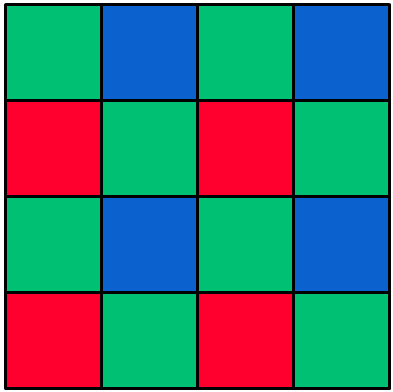
\includegraphics[width=0.3\textwidth]{Bayer1}
\caption{The Bayer pattern image resultant from the bayer filter capture.}
\label{Bayer1}
\end{figure}
 
\begin{figure}[!h]
\centering
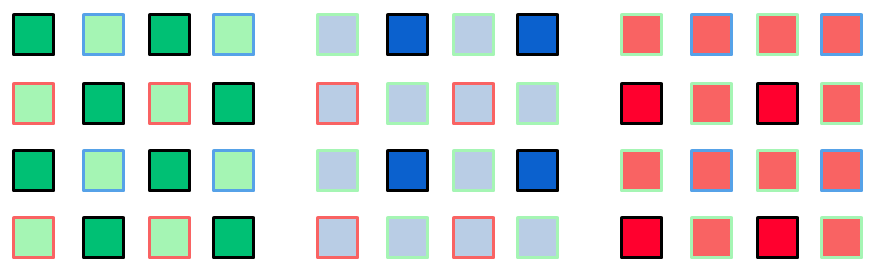
\includegraphics[width=0.9\textwidth]{Bayer2}
\caption{Descriptive diagram of the demosaicking to create the RGB channels from the Bayer pattern image.}
\label{Bayer2}
\end{figure}

The dark boxes in Figure \ref{Bayer2} represent the captured pixel while the lighter boxes are the interpolated locations, with their border showing what color was captured there. Again, there are twice as many green values as blue and red, but all three values are used at their captured spatial locations and then are interpolated to create a three channel RGB image.

Demosaicking is a well-understood and well-researched topic of interest where theories are being developed and applied to improve the interpolation results. The point to grasp here is that color imagery, even before any image processing algorithms are applied, is a sampled, quantized, and interpolated array of data. This shows a significant limitation in the strict accuracy of the initial information within a digital color image. While by no means a crippling factor, understanding this process allows for developing more scientifically stringent arguments for the concessions made later on in the development of the algorithm. For example, given this initial information loss in image capture, multiple-views are developed from statistically (randomly varied) quantized projections of the scene. Parallax and occlusion variations will occur with views at different spatial locations, but this also shows that intensity and color variations will occur in spite of any spatial variation. The views are inherently non-identical in terms of intensity/color, even when capturing the exact same object at the exact same depth and angle. This will be developed further as an important concept of the usefulness of limitations on the metric for the algorithm. There will be many assumptions and simplifications presented as part of the development of this algorithm, and by understanding them as progressing in a foundational manner, starting with those in the imaging system itself, a clear and applicable argument for the choices made in the development of this algorithm will be presented.

Therefore, at this stage, a digital image is seen initially as the demosaicked (interpolated) result of the Bayer pattern image. Stemming from that, a digital image is understood as a rigid, rectangular array of variable bit and channel depth. The number of channels pertains to the color range and the bit depth pertains to the intensity range. Standard contemporary color images are 3-channel (RGB) arrays of the notational size: $\mathfrak{m}\times\mathfrak{n}\times\mathfrak{p}$ (rows-by-columns-by-channels), and have a per pixel bit-depth of 8-bits, resulting in the descriptor of a 24-bit (3-channels with 8-bits each) color image. Variations of these characteristics exist in widespread use, and are important to understand, but the fundamental developments being made here can be easily translated to other image color-types and bit depths, thus all images in the rest of this work will be assumed 8 bits-per-pixel (bpp), 3-channel RGB images. But, the most fundamentally important concept in order to maintain a successful grasp of image processing is the notion that a digital image of size $\mathfrak{m} \times \mathfrak{n} \times \mathfrak{p}$ is akin to a $\mathfrak{p}$-dimensional discrete-space random variable.

Simplifying the discussion to the notion of an $\mathfrak{m} \times \mathfrak{n} \times 1$, henceforth $\mathfrak{m} \times \mathfrak{n}$, image, the functional definition of this image will be: $f(x,y)$. In the image space, $x$ refers to the column-axis and $y$ refers to the row-axis, meaning that the pixel location $(y_{i},x_{j})=(3,4)$ equates to row 3 and column 4, starting from the top left corner of the image (as per the MATLAB\textsuperscript{\textregistered} conventions). Note that $y$ and $x$ are not random vectors, they are independent vectors in either the image (frame) domain in the integer ranges: $[1,\mathfrak{n}]$ and $[1,\mathfrak{m}]$ respectively (again following MATLAB\textsuperscript{\textregistered} notation), or when shown as $\tilde{y}$ and $\tilde{x}$, they are in the global image (scene) domain with continuous ranges: $(-\infty,\infty)$ and $(-\infty,\infty)$. The world function (for the scene) will be denoted as $\tilde{f}(\tilde{x},\tilde{y})$, and is understood as a continuous function of the continuous space. Thus the digital image (a frame from the view of the scene) is known as a projected, sampled, and quantized version of the theoretical real world function (the proposed model of the scene), as mentioned previously. The approximating function's discrete result over the image domain, referred to for simplicity as the intensity image (a random variable), is thus a function of the set of discrete random outcomes of the image capture (the experiment). These terms follow from \cite{Papoulis2002} where the capturing of the light reflected off the scene is understood as the \textbf{experiment}. Each pixel is the projected, sampled, and quantized intensity of that light, and is understood as the \textbf{outcome} of the \textbf{experiment}. Thus the image that is formed can be seen as a function on those intensities and is therefore known as the \textbf{random variable}. The captured image is the two-dimensional (2-D) ($\mathfrak{m}\times\mathfrak{n}$) discrete random variable that is the projected, sampled, and quantized version of the continuous random variable (function) that describes the scene.

Thus as random variables, the images of a scene each have their own Probability Mass Function (PMF) which characterizes them \cite{Papoulis2002}. Though in our discussion we are making the assertion that the Probability Density Function (PDF) that describes the model random variable of the scene is being approximated by the PMF of the image that captures that scene. Each distinct view of the scene should be modeled by a distinct function of the intensities reflected and refracted by the objects in the scene, thus a distinct continuous random variable that will be approximated through image capture by the discrete random variable (image) associated with that view. And so the fundamental assertion being made is that overlapping views should share the same scene model in the overlap. Essentially describing two overlapping views as two random variables with non-trivial conditional probabilities. They are related and can describe each other, in part, because they are captured from the same original model, in that overlap region. And so a joint PMF between two overlapping views will be non-trivial and non-separable, asserting that distinct overlapping views are not independent. This is the foundation for the use of the mutual information metric. Non-mutually exclusive random variables will have some amount of mutual information between them.

And so to finalize the notation and understanding, the discussion is focused on the images captured from the scene. Each view generates an image ($f_{i}$) that is a 2-D random variable over the image domain (from $(1,1)$ to $(\mathfrak{m},\mathfrak{n})$). Each image has come from a projection, sampling, and quantization of the scene at that view that is modeled by $\tilde{f}_{i}$. The scene view has the PDF $\tilde{p}_{i}$ while the image from the view has the PMF $p_{i}$. The rest of the algorithm is built on the registration of two frames, extensible to multiple frames, and so the two images will be described more simply as random variables $A$ and $B$. Thus they will have a joint probability mass of $p_{AB}(\bf{a},\bf{b})$ and their marginal probability masses $p_{A}(\bf{a})$ and $p_{B}(\bf{b})$, where $\bf{a}$ and $\bf{b}$ are the outcomes (the vectors of intensities or feature values at the respective pixel locations). The 1-D PMF for digital images is accepted in practice as the normalized intensity histogram, and the 2-D Joint PMF is the normalized bi-variate intensity histogram. The next section will discuss the relationship between the image histogram and the proposed PMF notation, which will be used to characterize an image (the random variable) and its relationship to the corresponding scene.



%%%%%%%%%%%%%%%%%%%%%%%%%%%%%%%%%%%%%%%%%%%%%%%%%%%%%%%%%%%%%%%%%%%%%%%%%%%%%%%
% END OF DOCUMENT

